\begin{savequote}[75mm] 
And your heart hurts, mine does too\\
And it's just words and they cut deep
\qauthor{``Look What You've Done''- Drake} 
\end{savequote}

\chapter{Predicting Artist Influence with Siamese Networks}
Due to the limitations of the Document Influence Model, the need for richer feature representations and the scale of the audio dataset we collected, we next decided to investigate the application of deep learning, specifically an architecture known as a siamese convolutional neural network in modeling song-level influence. 

We address the following binary classification task: given as input a pair of two songs, what is the probability that there exists an influence relationship between the two artists who respectively recorded the songs?

\section{Model}
\subsection{Overview}
For the siamese network, we adopt a similar architecture as used by Koch et al. \cite{koch2015siamese} in predicting image similarity. Originally used for predicting similarity of two input images where the total number of image classes is large and the number of training instances for each class is sparse, siamese networks have been shown to be very successful in learning powerful descriptive features which generalize well to unseen pairs.

At a high level, our model takes in as input two mel-spectrogram representations of songs, which can essentially be viewed as ``images'' of the songs. Each of these inputs is fed separately through two copies of the same convolutional neural network (CNN). These two ``twin'' (hence the name siamese) CNNs extract a high-level fixed-length vector representation for each of the songs. The component-wise absolute distances between the extracted vectors for each of the songs are calculated, fed through a fully-connected perceptron layer, and then a sigmoid activation function is applied to output a probability between 0 and 1. A diagram of the model we used, including the input and output shapes for each layer, can be seen in the figure below:

\begin{figure}[H]
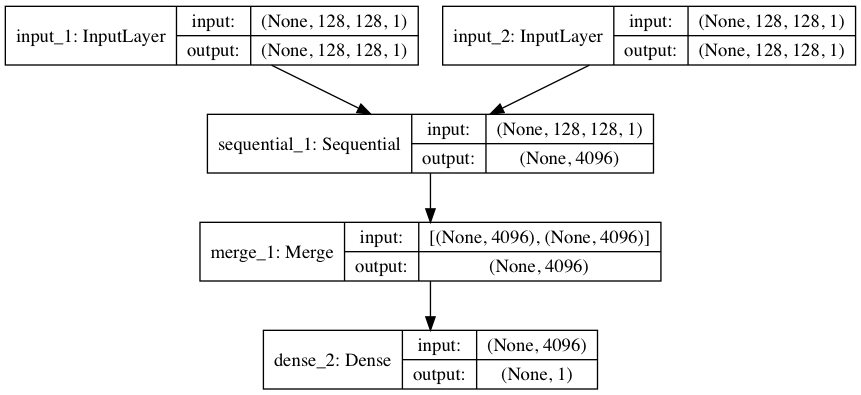
\includegraphics[width=\textwidth]{figures/siamese.png}
\caption{Diagram of siamese network architecture}
\end{figure}

\texttt{input\_1} and \texttt{input\_2} correspond to the 2 mel-spectrogram snippets of an input pair that we take in. A note on dimensions, taking the input dimensions of \texttt{input\_1}, $(None, 128,128,1)$ as an example: The first dimension corresponds to batch size, which was left as $None$ in the diagram for the sake of generality. The second and third dimensions correspond to the fact that each mel-spectrogram snippet used is a 128x128 matrix of real-valued numbers. The fourth dimension corresponds to the number of channels in the image, which was simply $1$ in our case (in color image applications for instance, channel size is commonly set to $3$ to deal with the RGB channels separately).

Each of the inputs are separately fed into the same CNN, called \texttt{sequential\_1} in our diagram for feature extraction. Shortly, we will discuss this CNN in further detail.

\texttt{sequential\_1} extracts a fixed-length vector representation of each song. In \texttt{merge\_1} the absolute element-wise differences between the vector representations for each song are calculated, and then in \texttt{dense\_2} the output is passed through one last fully connected layer with learnable weights, and a sigmoid activation function is applied.

The parameters for each of the layers of our siamese network are trained using the standard backpropagation algorithm against the standard binary cross-entropy loss function.

We implemented the model using the Keras library\cite{chollet2015keras} in Python.

\subsection{CNN Architecture}
We now give a more detailed description of the CNN architecture we used (\texttt{sequential\_1} in the figure above), depicted in detail in the figure below:

\begin{figure}[H]
\centering
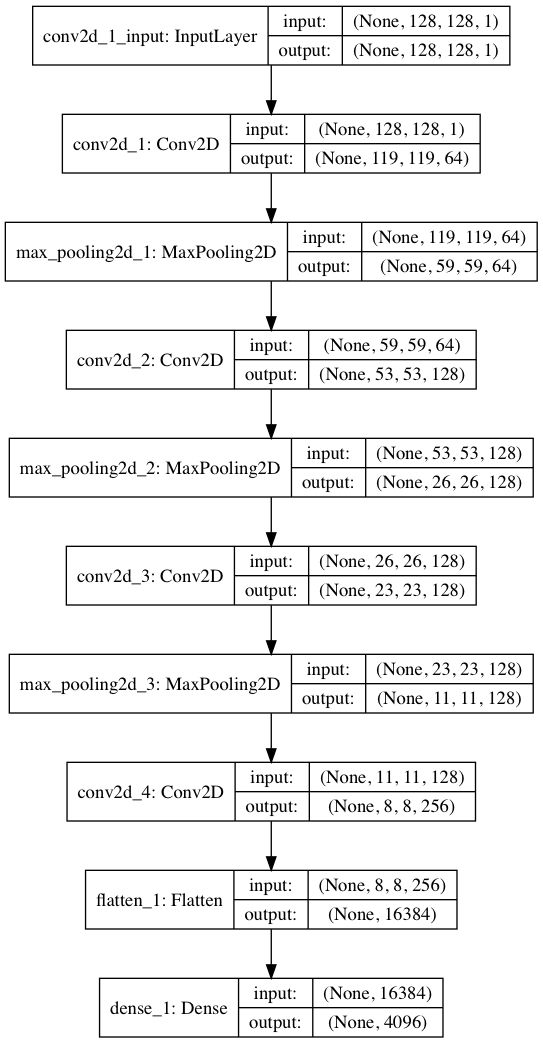
\includegraphics[width=8cm]{figures/conv_net.png}
\caption{Diagram of CNN architecture}
\end{figure}

Our CNN architecture consists of 4 convolutional layers with ReLU activation function, alternated with 3 max pooling layers. The first convolutional layer consists of 64 10x10 convolutional filters, the second convolutional layer consists of 128 7x7 filters, the third convolutional layer consists of 128 4x4 filters, and the fourth convolutional layer consists of 256 4x4 filters. Max pooling is performed in between convolutional layers in order to downsample the image. Finally the results from the last convolutional layer are flattened and passed through a fully-connected layer with the sigmoid activation function before being passed to \texttt{merge\_1} for calculation of distance between the feature vector representations for each song.



\section{Experimental Setup}

\subsection{Sampling of Songs}
Due to RAM limitations with the GPU we had access to for training and the need for reasonable training time, we were not able to use the entire mel-spectrogram representation corresponding to the full 30 seconds of audio we had access to for each song. Instead during training we randomly sampled contiguous 3 second samples on the fly from the full mel-spectrogram during each epoch (thereby generating different 3 second samples for each particular song each new epoch). Though using the full mel-spectrogram would have preserved the most information, given that previously \cite{van2013deep} 3 second samples have been used in other music audio tasks involving deep learning and our eventual results, this was likely a reasonable simplification.

In addition to sampling at the song-level, to further simplify training time, we only used the audio from one song for each artist despite having audio for up to 10 songs for most of the artists.

\subsection{Train-Validation Split}
As with any binary classification task, balance between the positive and negative example classes was a concern. In this case, our positive examples were derived from the ground truth AllMusic influence graph. Specifically, out of all edges in the ground truth graph, we had audio corresponding to 88,853 of them, and we used these pairs as our positive examples. We artificially generated negative examples of pairs where influence does not exist by randomly sampling for 88,853 artist pairs that do not correspond to edges in the ground truth graph, thereby creating a balanced number of positive and negative pairs overall. These combined 177,706 pairs were then randomly split into 80\% training and 20\% validation data. 

\subsection{Training}
Training was performed on a Tesla K20Xm GPU on Harvard's Odyssey cluster. We used a batch size of 16 and the Adam optimizer \cite{kingma2014adam} (an adaptive variant of standard Stochastic Gradient Descent), with training concluding after validation loss stopped decreasing for 5 epochs. In total, training took 51 epochs. 

\section{Results}
The loss and accuracy curves on both the training and validation sets can be seen in the figures below:

\begin{figure}[H]
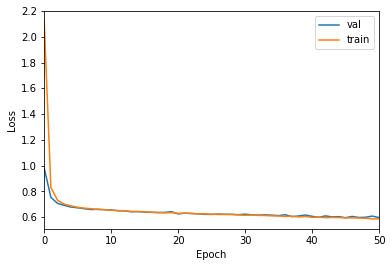
\includegraphics[width=\textwidth]{figures/loss.png}
\caption{Plot of loss curves for siamese network}
\end{figure}

\begin{figure}[H]
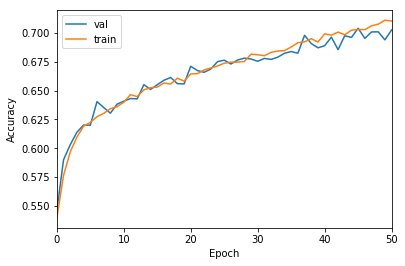
\includegraphics[width=\textwidth]{figures/accuracy.png}
\caption{Plot of accuracy curves for siamese network}
\end{figure}

On the validation set, the final model had an accuracy of $0.7005$. For comparison, due to the balanced nature of our dataset, a completely random model (using the result of a fair coin flip to guess whether an influence relationship exists or not between two input songs) would have had an accuracy of approximately $0.5$. Other metrics for the final model are summarized in the table below:

\begin{table}[H]
\centering
\caption{Accuracy metrics for trained siamese network on validation set}
\label{my-label}
\begin{tabular}{|l|l|}
\hline
Metric    & Value  \\ \hline
Accuracy  & 0.7005 \\ \hline
Precision & 0.6875 \\ \hline
Recall    & 0.7353 \\ \hline
F1 Score  & 0.7106 \\ \hline
\end{tabular}
\end{table}


\subsection{Same-Song Sample Prediction}
As a sanity check, we also tested the model's accuracy by creating pairs of samples where both samples were from the same song. Despite not being trained on this task, the model had an accuracy of $0.9018$ for identifying that the samples were from the same song.

\subsection{Intergenre vs. Intragenre Prediction}
We evaluated accuracy, precision and recall for intergenre v. intragenre prediction, using artist genre metadata information we gathered from AllMusic. Intergenre is defined as the two songs in the pair coming from artists of different genres (i.e. Jazz v. Classical) and intragenre is defined as sharing the same genre. The results are summarized in the table below:

\begin{table}[H]
\centering
\caption{Accuracy metrics for intergenre vs. intragenre prediction}
\label{my-label}
\begin{tabular}{|l|l|l|}
\hline
Metric    & Same Genre & Different Genre \\ \hline
Accuracy  & 0.7134     & 0.6971          \\ \hline
Precision & 0.8484     & 0.4198          \\ \hline
Recall    & 0.7676     & 0.6471          \\ \hline
F1 Score  & 0.8060     & 0.5092          \\ \hline
\end{tabular}
\end{table}

We see that across all metrics, the model outperforms on prediction when both artists are from the same genre vs. when the two artists are from different genres. In particular, we see that precision greatly suffers when the artists are from different genres.

% \subsection{TODO: Examples of Nearest Neighbor Songs}

\section{Discussion}
\subsection{Comparison to Morton and Kim}
Morton and Kim \cite{morton2015acoustic} used deep belief networks \cite{hinton2006fast} as feature extractors from spectral representations of songs before using logistic regression for classification. They treated influence prediction as a multi-label classification problem with 10 total classes, using the top 10 most influential artists from AllMusic in terms of outdegree as the classes. They achieved an F1-Score of approximately 0.4, though it is important to note that their results cannot directly be compared with ours due to differences in problem setup.

In contrast, our system using siamese convolutional neural networks is arguably more general. Instead of having a fixed number of artists as possible labels, our model takes in as input a pair of samples of songs and returns a binary prediction for whether there exists an influence relationship or not. This allows for extension to prediction on pairs where neither artist was seen during model training and therefore our model is a step closer to being an influence discriminator in a more general sense.

\subsection{Limitations}
The primary limitation of our method perhaps is the size of the samples used in training (3 second clips as opposed to the full 30 seconds we had available). We simply did not have the computational resources to use longer samples and still have the model train within a reasonable amount of time. Our model seems to have performed well even despite the short length of the samples, and this is perhaps plausible when one considers that when a human adjusts a radio dial, he/she is often able to figure out within seconds what he/she is listening to and whether to switch to the next station. That said, since music operates on several structural timescales, there is without a doubt information loss from such a limited timescale that our model is unable to account for.

In terms of information loss, we also only sampled one of the 10 tracks that we scraped per artist, and then further sampled a 3 second segment from that in the creation of our training pairs. One question then (which we were unable to address) is, given multiple audio samples per artist, how do we choose which ones to use when generating training pairs? After all, even if there exists an influence relationship between two artists, this might not be necessarily reflected in every song pairing consisting of a sample from each of the respective artists. A related question is, even assuming that one has a sufficiently ``good'' feature representation of a song (e.g. extracted from a CNN), how does one go from song level summarizations to an artist-level summarization? Obviously, certain heuristics such as averaging come to mind, but is there a more robust way? All of these remain open questions.
